\documentclass[10pt]{beamer}

\usetheme{metropolis}

\usepackage[export]{adjustbox}
\usepackage{array}
\usepackage{bbm}
\usepackage{etoolbox}
\usepackage{graphicx}
\usepackage{hyperref}
\usepackage{listings}
\usepackage{pgfplots}
\usepackage{tikz}
\usepackage{xcolor}

\usepgfplotslibrary{fillbetween}

\usetikzlibrary{arrows.meta}
\usetikzlibrary{calc}
\usetikzlibrary{patterns}

\hypersetup{
    colorlinks=true,
    linkcolor=white,
    urlcolor=blue!80
}

\definecolor{uiored}{HTML}{DD0000}
\definecolor{uiolightred}{HTML}{FB6666}
\definecolor{uioredtone}{HTML}{FEE0E0}
\definecolor{uioblue}{HTML}{3E31D6}
\definecolor{uiolightblue}{HTML}{86A4F7}
\definecolor{uioblueone}{HTML}{E6ECFF}
\definecolor{uiogreen}{HTML}{2EC483}
\definecolor{uiolightgreen}{HTML}{6CE1AB}
\definecolor{uiogreentone}{HTML}{CEFFDF}
\definecolor{uioorange}{HTML}{FEA11B}
\definecolor{uiolightorange}{HTML}{FDCB87}
\definecolor{uioorangetone}{HTML}{FFE8D4}
\definecolor{uioyellow}{HTML}{FFFEA7}
\definecolor{uiogray}{HTML}{B2B3B7}

\colorlet{mainbackground}{uiored}

\setbeamercolor{frametitle}{bg=mainbackground, fg=white}
\setbeamercolor{title separator}{fg=mainbackground}
\setbeamercolor{progress bar in section page}{fg=white, bg=uiogray}

\def\logowidth{4cm}

\makeatletter
\setbeamertemplate{section page}
{
  \begingroup

    \vspace{4.3cm}
    {\usebeamercolor[fg]{section title}\usebeamerfont{section title}\insertsectionhead}\\[-1ex]
    {\centering\color{white}\rule{\linewidth}{1pt}\par} % the horizontal line

    \vspace*{3.1cm}
    \begin{center}
        
\includegraphics[width=\logowidth,valign=c]{data/uio_logo_full_white.png} % Adjust width and path to your logo as needed
    \end{center}

  \endgroup
}
\makeatother

\AtBeginSection{
  {
    \setbeamercolor{background canvas}{bg=uiored}
    \setbeamercolor{section title}{fg=white}
    \frame[plain,c,noframenumbering]{\sectionpage}
    \setbeamercolor{background canvas}{bg=black!2}
  }
}



\setbeamertemplate{footline}{
    \ifnum\insertframenumber=1
        % Title page, no footer
    \else
        \begin{tikzpicture}[remember picture,overlay]
            \fill[mainbackground] (current page.south west) rectangle ([yshift=0.45cm]current page.south east); % Draw filled rectangle

            % Logo
            \node[anchor=west, yshift=0.225cm] at (current page.south west) {
\includegraphics[height=1.2cm]{data/uio_logo_white.png}};

            % Title and subtitle
            \node[align=center, yshift=0.225cm] at (current page.south) {\textcolor{white}{\textbf{\inserttitle}}\\[0.05cm]\textcolor{white}{\insertsubtitle}};

            % Page number
            \node[anchor=east, yshift=0.225cm, xshift=-0.2cm, align=right] at (current page.south east) {\textcolor{white}{\insertframenumber/\inserttotalframenumber}};
        \end{tikzpicture}
    \fi
}

\lstdefinestyle{Core}{
    identifierstyle=\color[RGB]{0, 0, 0},
    stringstyle=\color[RGB]{205, 49, 49},
    showstringspaces=false,
    breaklines,
    xleftmargin=3pt,
    xrightmargin=3pt,
    framesep=3pt,
    aboveskip=-1.5pt,
    belowskip=-0.5pt,
    showlines=true,
}

\lstdefinestyle{RInput}{
    style=Core,
    language=R,
    keywordstyle=\color[RGB]{17, 115, 187},
    commentstyle=\color[RGB]{0, 128, 0},
    identifierstyle=\color[RGB]{0, 0, 0},
    stringstyle=\color[RGB]{205, 49, 49},
    backgroundcolor=\color[RGB]{255, 255, 255},
    frame=single,
    rulecolor=\color[RGB]{0, 0, 0},
}

\lstdefinestyle{PythonInput}{
    style=Core,
    language=Python,
    keywordstyle=\color[RGB]{26, 13, 171},
    commentstyle=\color[RGB]{0, 128, 0},
    backgroundcolor=\color[RGB]{245, 245, 245},
    rulecolor=\color[RGB]{192, 192, 192},
    frame=tblr,
}

\lstdefinestyle{ROutput}{
    style=Core,
    language=R,
    backgroundcolor=\color[RGB]{255, 255, 255},
    commentstyle=\color[HTML]{009900},
    stringstyle=\color[HTML]{0000FF},
    keywordstyle=\color[HTML]{000000},
    numberstyle=\tiny\color[HTML]{000000},
    breakatwhitespace=true,
    frame=single,
    rulecolor=\color{black},
}

\lstdefinestyle{PythonOutput}{
    backgroundcolor=\color[RGB]{255, 255, 255},
    rulecolor=\color[RGB]{192, 192, 192},
    frame=single,
    numbers=none,
    showstringspaces=false,
    breakatwhitespace=true,
    keywordstyle=\color[RGB]{255, 0, 0},
    morekeywords={AttributeError}
}

\newcommand{\PythonInputNode}[6]{%
    \node[
        minimum width=#4,
        text width=#4,
        align=left,
        inner sep=0pt,
        outer sep=0pt,
        anchor=north west,
        label={[blue,
                anchor=north east,
                font=\ttfamily\fontsize{\the\numexpr#5-1\relax}{#5}\selectfont,
                inner sep=0pt,
                outer sep=0pt,
                xshift=-3pt,
                yshift=-3pt
                ]north west:In{[}#1{]}:},
    ] (#3) at #2 {
    \begin{lstlisting}[
        style=PythonInput,
        linewidth=#4,
        basicstyle=\ttfamily\fontsize{\the\numexpr#5-1\relax}{#5}\selectfont,
        numberstyle=\fontsize{\the\numexpr#5-1\relax}{#5}\selectfont\color[RGB]{128, 128, 128},
    ]^^J
        #6
    \end{lstlisting}
    };
}

\newcommand{\RInputNode}[5]{
    \node[
        minimum width=#3,
        text width=#3,
        align=left,
        inner sep=0pt,
        outer sep=0pt,
        draw=black,
        anchor=north west
    ] (#2) at #1 {
        \begin{lstlisting}[
            style=RInput,
            linewidth=\textwidth,
            basicstyle=\ttfamily\fontsize{\the\numexpr#4-1\relax}{#4}\selectfont,
            numberstyle=\fontsize{\the\numexpr#4-1\relax}{#4}\selectfont\color[RGB]{128, 128, 128},
        ]^^J
            #5
        \end{lstlisting}
    };
}

\title{PSY9511: Seminar 4}
\subtitle{The basics of regression and classification}
\author{Esten H. Leonardsen}
\date{29.05.2024}

\titlegraphic{
	\centering
	\vspace{7.7cm}
	
\includegraphics[width=\logowidth]{data/uio_logo_full.png}
}

\begin{document}
	\begin{frame}
	 	\titlepage
	\end{frame}

    \begin{frame}[t]{Recap}
        \only<1-4>{
            \vspace{0.5cm}
            \underline{What is statistical learning?}\\
            \vspace{0.5cm}


            \only<2>{\small{\textbf{Inferentiental view:} Finding a function $\hat{f}(X)$ that describes the relationship between some input variables $X$ and an output variable $y$.}\\}
            \only<3>{\textcolor{gray!20}{\small{\textbf{Inferentiental view:} Finding a function $\hat{f}(X)$ that describes the relationship between some input variables $X$ and an output variable $y$.}\\}}
            \only<4>{\small{\textcolor{gray!20}{\textbf{Inferentiental view:}} Finding a function $\hat{f}(X)$ \textcolor{gray!20}{that describes the relationship between some input variables $X$ and an output variable $y$.}\\}}
            \vspace{0.25cm}
            \vspace{0.25cm}
            \only<3>{\small{\textbf{Predictive view:} Finding a function $\hat{f}(X)$ that, when given a new set of inputs $X$ allows us to predict an output $y$.}}
            \only<4>{\small{\textcolor{gray!20}{\textbf{Predictive view:}} Finding a function $\hat{f}(X)$ \textcolor{gray!20}{ that, when given a new set of inputs $X$ allows us to predict an output $y$.}}}
        }

        \onslide<5->{
            \centering
            \begin{tikzpicture}
                \begin{axis}[
                    xtick pos=bottom,
                    ytick pos=left,
                    xmin=30,
                    xmax=240,
                    ymin=3,
                    ymax=50,
                    xlabel=Horsepower (x),
                    ylabel=Miles per gallon (y),
                    height=6.8cm,
                    width=11cm
                ]
                    \addplot[
                        only marks,
                        opacity=0.6
                    ] table [
                        col sep=comma,
                        x=horsepower,
                        y=mpg
                    ] {data/Auto.csv};
                    \only<7>{
                        \addplot[
                            domain=30:240,
                            samples=100,
                            color=red,
                            thick
                        ] {39.93 - 0.1578*x};
                    }
                    \only<8>{
                        \addplot[
                            domain=30:240,
                            samples=100,
                            color=red,
                            thick
                        ] {23.44};
                    }
                    \only<9>{
                        \addplot[
                            domain=30:240,
                            samples=100,
                            color=red,
                            thick
                        ] {exp(3.86-0.0073*x)};
                    }
                \end{axis}
            \end{tikzpicture}\\
            \vspace{0.2cm}
            \hspace{1.3cm}
            \only<6>{
                \textcolor{red}{$\hat{y}=\hat{f}(x)$}
            }
            \only<7>{
                \textcolor{red}{$\hat{y}=39.93-0.1578x$}
            }
            \only<8>{
                \textcolor{red}{$\hat{y}=23.44$}
            }
            \only<9>{
                \textcolor{red}{$\hat{y}=e^{3.86-0.0073x}$}
            }
        }
    \end{frame}

    \begin{frame}[t]{Outline}
        \underline{Plan for the day:}
        \begin{itemize}
            \item Different types of outputs $y$: Regression vs classification
            \item Linear regression: Restricting the scope of $\hat{f}(X)$
            \begin{itemize}
                \item Finding $\hat{f}(X)$: Training machine learning models
                \item Live coding
            \end{itemize}
            \item k Nearest Neighbours
            \item Logistic regression: Extending linear regression to classification
            \begin{itemize}
                \item Live coding
            \end{itemize}
            \item Generative models
        \end{itemize}

        \underline{Plan for future lectures:}
        \begin{itemize}
            \item How do we evaluate how good our models are? (Lecture 3)
            \item Complex solutions to regression and classification problems (Lecture 4 and onwards)
        \end{itemize}
    \end{frame}

    \newcommand{\weightnode}[3]{
        \node[circle, draw=black, fill=teal!60, opacity=#3] at (#1, #2*3.5) {};
    }

    \newcommand{\weightplot}[1]{
        \begin{tikzpicture}
            \ifnum#1<3
                \draw[|-Latex] (0, 3.3*3.5) -- (0, 4.6*3.5);
                \weightnode{0}{3.850}{1.0}
                \weightnode{0}{4.354}{1.0}
            \fi
            \ifnum#1>2
                \draw[|-Latex,black!20] (0, 3.3*3.5) -- (0, 4.6*3.5);
                \weightnode{0}{3.850}{0.2}
                \weightnode{0}{4.354}{0.2}
            \fi
            \ifnum#1=1
                \weightnode{0}{3.504}{1.0}
                \weightnode{0}{3.693}{1.0}
                \weightnode{0}{3.436}{1.0}
                \weightnode{0}{3.433}{1.0}
                \weightnode{0}{3.449}{1.0}
                \weightnode{0}{4.341}{1.0}
                \weightnode{0}{4.354}{1.0}
                \weightnode{0}{4.312}{1.0}
                \weightnode{0}{4.425}{1.0}
            \fi
            \ifnum#1>1
                \weightnode{0}{3.504}{0.2}
                \weightnode{0}{3.693}{0.2}
                \weightnode{0}{3.436}{0.2}
                \weightnode{0}{3.433}{0.2}
                \weightnode{0}{3.449}{0.2}
                \weightnode{0}{4.341}{0.2}
                \weightnode{0}{4.354}{0.2}
                \weightnode{0}{4.312}{0.2}
                \weightnode{0}{4.425}{0.2}

                \ifnum#1=2
                    \draw[|-|, dashed] (0.5, 3.850*3.5) -- (0.5, 4.354*3.5);
                    \node[anchor=west] at (0.5, 4.102*3.5) {\small{504}};
                \fi
            \fi
        \end{tikzpicture}
    }

    \newsavebox{\weightboxfirst}
    \sbox{\weightboxfirst}{
        \weightplot{1}
    }

    \newsavebox{\weightboxsecond}
    \sbox{\weightboxsecond}{
        \weightplot{2}
    }

    \newsavebox{\weightboxhidden}
    \sbox{\weightboxhidden}{
        \weightplot{3}
    }

    \newcommand{\manufacturernode}[5]{
        \node[circle, draw=black, fill=#3, opacity=#4] (#5) at (#1, #2) {};
    }


    \newcommand{\manufacturerplot}[1]{
        \begin{tikzpicture}
            \colorlet{chewy}{blue!60}
            \colorlet{ford}{red!60}
            \colorlet{pontiac}{green!60}

            \manufacturernode{0}{0}{chewy}{1.0}{c0}
            \manufacturernode{1}{-1.2}{ford}{1.0}{f0}
            \manufacturernode{-0.3}{-1.1}{pontiac}{1.0}{p0}

            \ifnum#1=1
                \manufacturernode{0.5}{0.4}{chewy}{1.0}{}
                \manufacturernode{0.1}{0.5}{chewy}{1.0}{}

                \manufacturernode{1.4}{-1.0}{ford}{1.0}{}
                \manufacturernode{1.5}{-1.5}{ford}{1.0}{}
                \manufacturernode{0.9}{-1.6}{ford}{1.0}{}

                \manufacturernode{-0.1}{-1.5}{pontiac}{1.0}{}
                \manufacturernode{0.2}{-1.05}{pontiac}{1.0}{}
            \fi
            \ifnum#1=2
                \manufacturernode{0.5}{0.4}{chewy}{0.2}{}
                \manufacturernode{0.1}{0.5}{chewy}{0.2}{}

                \manufacturernode{1.4}{-1.0}{ford}{0.2}{}
                \manufacturernode{1.5}{-1.5}{ford}{0.2}{}
                \manufacturernode{0.9}{-1.6}{ford}{0.2}{}

                \manufacturernode{-0.1}{-1.5}{pontiac}{0.2}{}
                \manufacturernode{0.2}{-1.05}{pontiac}{0.2}{}

                \draw[->, dashed] (c0) -- (f0) node[pos=0.7, above=0.15cm] {\footnotesize{?}};
                \draw[->, dashed] (c0) -- (p0) node[pos=0.9, above=0.2cm] {\footnotesize{?}};;
            \fi

            \node[anchor=south] at (0.25, 0.7) {\textbf{\small{Chevrolet}}};
            \node[anchor=north] at (1.2, -1.8) {\textbf{\small{Ford}}};
            \node[anchor=north] at (0.05, -1.7) {\textbf{\small{Pontiac}}};

        \end{tikzpicture}
    }

    \newsavebox{\manufacturerboxfirst}
    \sbox{\manufacturerboxfirst}{
        \manufacturerplot{1}
    }

    \newsavebox{\manufacturerboxsecond}
    \sbox{\manufacturerboxsecond}{
        \manufacturerplot{2}
    }

    \begin{frame}{Regression vs. classification}
        \only<1-5>{
            \begin{tikzpicture}
                \node[] at (-5.25, -3) {};
                \node[] at (5.25, 3) {};
                \only<1-2,4>{
                    \node[] at (0, 0) {
                        \begin{tabular}{cc}
                            \textbf{Weight}&\textbf{Manufacturer}\\
                            3504&Chevrolet\\
                            3693&Ford\\
                            3436&Pontiac\\
                            3433&Pontiac\\
                            3449&Ford\\
                            4341&Ford\\
                            4354&Chevrolet\\
                            4312&Ford\\
                            4425&Pontiac\\
                            3850&Chevrolet\\
                        \end{tabular}
                    };
                }
                \onslide<2,4>{
                    \node[anchor=west] at (-4, 0) {
                        \usebox{\weightboxfirst}
                    };
                }
                \only<3>{
                    \node[anchor=west] at (-4, 0) {
                        \usebox{\weightboxsecond}
                    };
                    \node[] at (0, 0) {
                        \begin{tabular}{cc}
                            \textbf{Weight}&\textcolor{gray!20}{\textbf{Manufacturer}}\\
                            \textcolor{gray!20}{3504}&\textcolor{gray!20}{Chevrolet}\\
                            \textcolor{gray!20}{3693}&\textcolor{gray!20}{Ford}\\
                            \textcolor{gray!20}{3436}&\textcolor{gray!20}{Pontiac}\\
                            \textcolor{gray!20}{3433}&\textcolor{gray!20}{Pontiac}\\
                            \textcolor{gray!20}{3449}&\textcolor{gray!20}{Ford}\\
                            \textcolor{gray!20}{4341}&\textcolor{gray!20}{Ford}\\
                            4354&\textcolor{gray!20}{Chevrolet}\\
                            \textcolor{gray!20}{4312}&\textcolor{gray!20}{Ford}\\
                            \textcolor{gray!20}{4425}&\textcolor{gray!20}{Pontiac}\\
                            3850&\textcolor{gray!20}{Chevrolet}\\
                        \end{tabular}
                    };
                }
                \only<4>{
                    \node[anchor=east] at (5, 0) {
                        \usebox{\manufacturerboxfirst}
                    };
                }
                \only<5>{
                    \node[anchor=west] at (-4, 0) {
                        \usebox{\weightboxhidden}
                    };
                    \node[anchor=east] at (5, 0) {
                        \usebox{\manufacturerboxsecond}
                    };
                    \node[] at (0, 0) {
                        \begin{tabular}{cc}
                            \textcolor{gray!20}{\textbf{Weight}}&\textbf{Manufacturer}\\
                            \textcolor{gray!20}{3504}&\textcolor{gray!20}{Chevrolet}\\
                            \textcolor{gray!20}{3693}&Ford\\
                            \textcolor{gray!20}{3436}&\textcolor{gray!20}{Pontiac}\\
                            \textcolor{gray!20}{3433}&\textcolor{gray!20}{Pontiac}\\
                            \textcolor{gray!20}{3449}&\textcolor{gray!20}{Ford}\\
                            \textcolor{gray!20}{4341}&\textcolor{gray!20}{Ford}\\
                            \textcolor{gray!20}{4354}&Chevrolet\\
                            \textcolor{gray!20}{4312}&\textcolor{gray!20}{Ford}\\
                            \textcolor{gray!20}{4425}&Pontiac\\
                            \textcolor{gray!20}{3850}&\textcolor{gray!20}{Chevrolet}\\
                        \end{tabular}
                    };

                }
            \end{tikzpicture}
        }
        \only<6>{
            \centering
            \begin{tikzpicture}
                \node[align=center, anchor=north] at (0.5, 0) {
                    \underline{\small{Mean squared error (MSE):}}\\[0.3cm]
                    $\frac{1}{n}\sum_{i=1}^{n}(y_i-\hat{y}_i)^2$
                };
                \node[align=center, anchor=north] at (6.5, 0) {
                    \underline{\small{Accuracy}}\\[0.3cm]
                    $\frac{1}{n}\sum_{i=1}^{n}\mathbbm{1}_{eq} (y_i,\hat{y}_i)$,\\
                    $\mathbbm{1}_{eq}(a, b)=\begin{cases}1 & \text{if } a=b\\0 & \text{if } a\neq b\end{cases}$
                };
            \end{tikzpicture}
        }
        \only<7>{

        }
        \only<8-9>{
            \centering
            \begin{tikzpicture}
                \node[] at (-4.5, 1) {};
                \node[] at (5.5, -4) {};
                \node[] (sentence) at (0, 0) {
                    The quick brown fox jumps over the lazy
                };
                \draw[red] ($ (sentence.south east) + (0, 0.15) $) -- ($ (sentence.south east) + (1, 0.15) $);
                \only<9>{
                    \draw (2,-2) ellipse (1.8cm and 0.9cm);
                    \node[] at (3, -2.4) {\footnotesize{cat}};
                    \node[] at (1, -2.2) {\textbf{\footnotesize{dog}}};
                    \node[] at (2.1, -1.6) {\footnotesize{hurdle}};
                    \node[] at (2, -3.3) {\small{Classification}};
                }
            \end{tikzpicture}
        }
        \only<10-11>{
            \centering
            \begin{tikzpicture}
                \node[] at (-5.5, 2) {};
                \node[] at (5, -4) {};

                \node[align=center] (prompt) at (-4, 0) {
                    "Students taking\\a machine learning\\class"
                };
                \node[fill=white, draw=black] (model) at (-1, 0) {
                    
\includegraphics[width=1cm]{data/chatgpt.png}
                };
                \node[] (output)at (2.5, 0) {
                    
\includegraphics[width=4cm]{data/ml-students.png}
                };
                \draw[-Latex] (prompt) -- (model);
                \draw[-Latex] (model) -- (output);

                \only<11>{
                    \node[draw=black, fill=red!50, inner sep=5pt, opacity=0.9] at (-2, -3) {};
                    \node[draw=black, fill=green!75, inner sep=5pt, opacity=0.9] (green) at (-1.9, -3.1) {};
                    \node[draw=black, fill=blue!25, inner sep=5pt, opacity=0.9] at (-1.8, -3.2) {};
                    \node[anchor=west] at ($ (green.east) + (0.2, 0) $) {(128, 192, 64)};
                }
            \end{tikzpicture}
        }
        \only<12>{
            \begin{tikzpicture}
                \node[anchor=west] at (0, 0) {
                    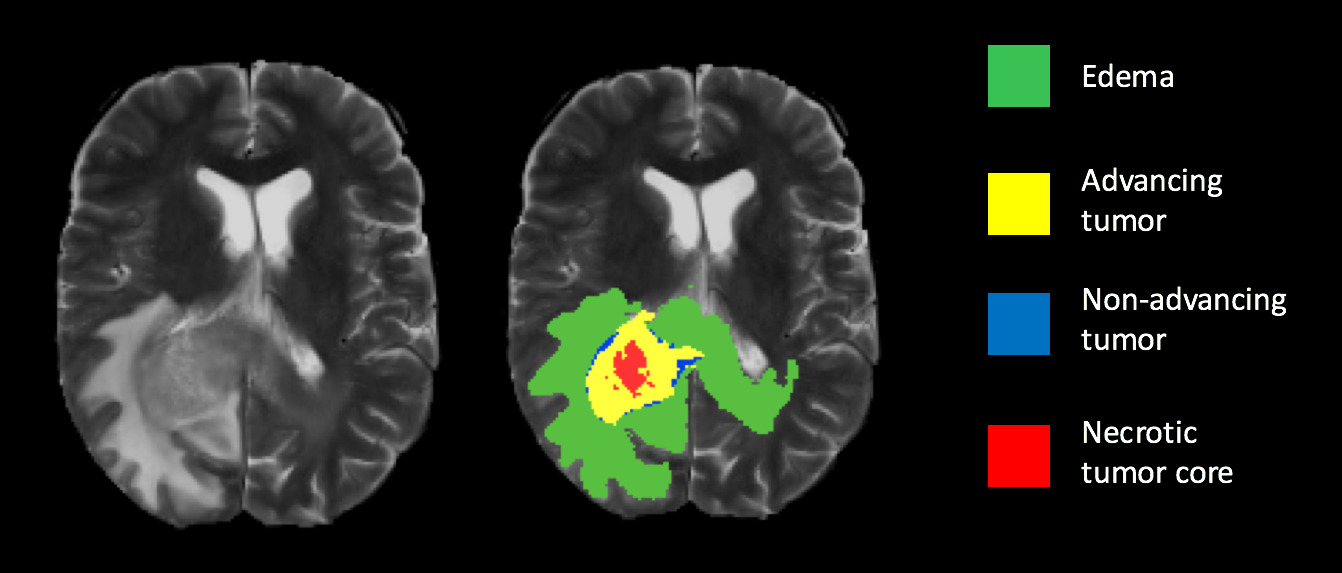
\includegraphics[
                        height=4.5cm,
                        trim={0 0 13.8cm 0},
                        clip
                    ]{data/tumor.png}
                };
            \end{tikzpicture}
        }
        \only<13>{
            \begin{tikzpicture}
                \node[anchor=west] at (0, 0) {
                    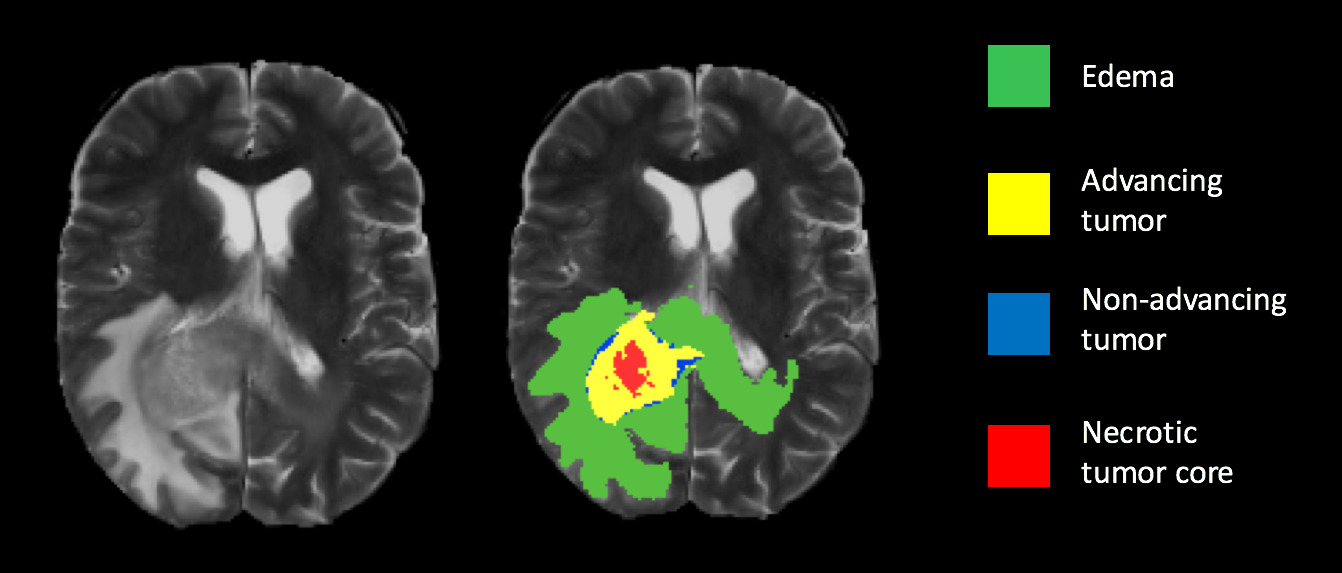
\includegraphics[height=4.5cm]{data/tumor.png}
                };
            \end{tikzpicture}
        }
    \end{frame}

    \newsavebox{\linreg}
    \sbox{\linreg}{
        \begin{tikzpicture}
            \begin{axis}[
                xmin=30,
                xmax=240,
                ymin=3,
                ymax=50,
                width=5.2cm,
                height=5.2cm,
                ylabel=mpg,
                xlabel=horsepower
            ]
                \addplot[
                    only marks,
                    opacity=0.3
                ] table [
                    col sep=comma,
                    x=horsepower,
                    y=mpg
                ] {data/Auto.csv};
                \addplot[
                    domain=30:240,
                    samples=100,
                    color=red,
                    thick
                ] {39.93 - 0.1578*x};
            \end{axis}
        \end{tikzpicture}
    }

    \newsavebox{\residuals}
    \sbox{\residuals}{
        \begin{tikzpicture}
            \begin{axis}[
                % xmin=30,
                % xmax=240,
                % ymin=3,
                % ymax=50,
                width=5.2cm,
                height=5.2cm,
                ylabel=$y-\hat{y}$,
                xlabel=horsepower
            ]
            \end{axis}
        \end{tikzpicture}
    }

    \newsavebox{\multilinreg}
    \sbox{\multilinreg}{
        \begin{tikzpicture}
            \begin{axis}[
                width=8cm,
                height=7cm, % Size of the plot
                xlabel={Horsepower ($x_1$)},
                ylabel={Weight ($x_2$)},
                zlabel={Miles per gallon (y)},
                view={45}{20}, % Adjust viewing angle colormap/cool,
                xmin=30,
                xmax=240,
                ymin=1500,
                ymax=5000,
                zmin=3,
                zmax=50,
                xlabel style={sloped},
                ylabel style={sloped}
            ]
                \addplot3[
                    only marks,
                    mark size=2.5pt, % Size of each point
                    opacity=0.5
                ] table [
                    x=horsepower,
                    y=weight,
                    z=mpg,
                    col sep=comma
                ] {data/Auto.csv};
                \addplot3[
                    surf,
                    opacity=0.5,
                    samples=20,
                    domain=30:240,
                    y domain=1500:5000,
                ] {45.64-0.04*x-0+.005*y}; % Replace this formula with your plane's equation
            \end{axis}
        \end{tikzpicture}
    }

    \newcommand{\binaryplot}[1]{
        \begin{tikzpicture}
            \begin{axis}[
                xmin=-0.5,
                xmax=1.5,
                xtick={0, 1},
                xticklabels={Ford, Chevrolet},
                ylabel=mpg,
                height=7cm,
                width=7cm
            ]
                \addplot[
                    only marks,
                    fill=blue,
                    opacity=0.6
                ] coordinates {
                    (-0.065, 18)
                    (-0.080, 15)
                    (-0.038, 18)
                    (-0.139, 16)
                    (0.028, 17)
                    (-0.140, 15)
                    (-0.149, 14)
                    (0.137, 14)
                    (0.043, 14)
                    (-0.101, 15)
                    (0.007, 15)
                    (-0.145, 14)
                    (-0.106, 15)
                    (-0.013, 14)
                    (-0.120, 24)
                    (0.150, 22)
                    (-0.166, 18)
                    (-0.052, 21)
                    (0.031, 27)
                };
                \addplot[
                    only marks,
                    fill=red,
                    opacity=0.6
                ] coordinates {
                    (0.985, 38)
                    (0.943, 36)
                    (1.085, 36)
                    (0.971, 36)
                    (0.990, 34)
                    (1.029, 38)
                    (0.958, 32)
                    (1.018, 38)
                    (1.054, 25)
                    (1.064, 38)
                    (1.070, 26)
                    (0.938, 22)
                    (1.131, 32)
                    (1.009, 36)
                    (0.835, 27)
                    (1.109, 27)
                    (1.032, 44)
                    (1.142, 32)
                    (1.115, 28)
                    (1.009, 31)
                };
                \ifnum#1=2
                    \draw[thick, dashed] (axis cs: -0.3, 17.158) -- (axis cs: 0.3, 17.158);
                    \node[anchor=south east, inner sep=1pt] at (axis cs: 0.3, 17.158) {\small{17.1}};
                    \draw[thick, dashed] (axis cs: 0.7, 32.8) -- (axis cs: 1.3, 32.8);
                    \node[anchor=south west, inner sep=1pt] at (axis cs: 0.7, 32.8) {\small{32.8}};
                \fi
            \end{axis}
        \end{tikzpicture}
    }

    \newsavebox{\binary}
    \savebox{\binary}{
        \binaryplot{1}
    }
    \newsavebox{\binarymeans}
    \savebox{\binarymeans}{
        \binaryplot{2}
    }

    \newsavebox{\multilevel}
    \savebox{\multilevel}{
        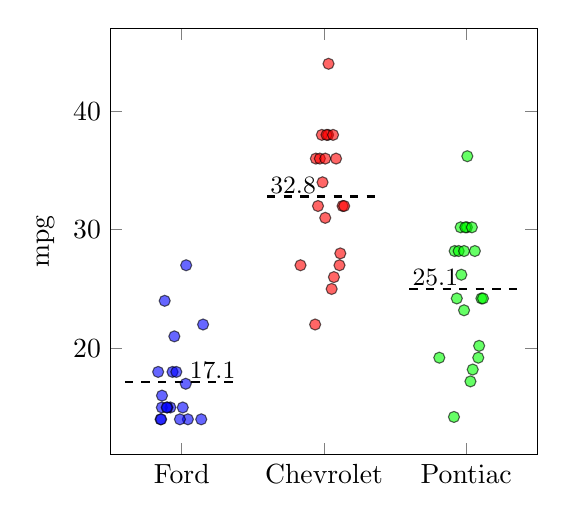
\begin{tikzpicture}
            \begin{axis}[
                xmin=-0.5,
                xmax=2.5,
                xtick={0, 1, 2},
                xticklabels={Ford, Chevrolet, Pontiac},
                ylabel=mpg,
                height=7cm,
                width=7cm
            ]
                \addplot[
                    only marks,
                    fill=blue,
                    opacity=0.6
                ] coordinates {
                    (-0.065, 18)
                    (-0.080, 15)
                    (-0.038, 18)
                    (-0.139, 16)
                    (0.028, 17)
                    (-0.140, 15)
                    (-0.149, 14)
                    (0.137, 14)
                    (0.043, 14)
                    (-0.101, 15)
                    (0.007, 15)
                    (-0.145, 14)
                    (-0.106, 15)
                    (-0.013, 14)
                    (-0.120, 24)
                    (0.150, 22)
                    (-0.166, 18)
                    (-0.052, 21)
                    (0.031, 27)
                };
                \addplot[
                    only marks,
                    fill=red,
                    opacity=0.6
                ] coordinates {
                    (0.985, 38)
                    (0.943, 36)
                    (1.085, 36)
                    (0.971, 36)
                    (0.990, 34)
                    (1.029, 38)
                    (0.958, 32)
                    (1.018, 38)
                    (1.054, 25)
                    (1.064, 38)
                    (1.070, 26)
                    (0.938, 22)
                    (1.131, 32)
                    (1.009, 36)
                    (0.835, 27)
                    (1.109, 27)
                    (1.032, 44)
                    (1.142, 32)
                    (1.115, 28)
                    (1.009, 31)
                };
                \addplot[
                    only marks,
                    fill=green,
                    opacity=0.6
                ] coordinates {
                    (1.961, 30.200)
                    (1.919, 28.200)
                    (2.061, 28.200)
                    (1.947, 28.200)
                    (1.966, 26.200)
                    (2.005, 30.200)
                    (1.934, 24.200)
                    (1.994, 30.200)
                    (2.030, 17.200)
                    (2.040, 30.200)
                    (2.046, 18.200)
                    (1.914, 14.200)
                    (2.107, 24.200)
                    (1.985, 28.200)
                    (1.811, 19.200)
                    (2.085, 19.200)
                    (2.008, 36.200)
                    (2.118, 24.200)
                    (2.091, 20.200)
                    (1.985, 23.200)
                };

                \draw[thick, dashed] (axis cs: -0.4, 17.158) -- (axis cs: 0.4, 17.158);
                \node[anchor=south east, inner sep=1pt] at (axis cs: 0.4, 17.158) {\small{17.1}};
                \draw[thick, dashed] (axis cs: 0.6, 32.8) -- (axis cs: 1.4, 32.8);
                \node[anchor=south west, inner sep=1pt] at (axis cs: 0.6, 32.8) {\small{32.8}};
                \draw[thick, dashed] (axis cs: 1.6, 25) -- (axis cs: 2.4, 25);
                \node[anchor=south west, inner sep=1pt] at (axis cs: 1.6, 25) {\small{25.1}};

            \end{axis}
        \end{tikzpicture}
    }

    \newcommand{\combinationplot}[1]{
        \begin{tikzpicture}
            \begin{axis}[
                xtick pos=bottom,
                ytick pos=left,
                xmin=30,
                xmax=240,
                ymin=3,
                ymax=50,
                xlabel=Horsepower,
                ylabel=Miles per gallon,
                height=6.5cm,
                width=10.5cm
            ]
                \addplot[
                    only marks,
                    opacity=0.6
                ] table [
                    col sep=comma,
                    x=horsepower,
                    y=mpg
                ] {data/Auto.csv};

                \ifnum#1=1
                    \addplot[
                        domain=30:240,
                        samples=100,
                        color=red,
                        thick
                    ] {40 - 0.1566*x};
                    \addplot[
                        domain=30:240,
                        samples=100,
                        color=blue,
                        thick
                    ] {40 - 0.1566*x-1.85};
                \fi
                \ifnum#1=2
                    \addplot[
                        domain=30:240,
                        samples=100,
                        color=red,
                        thick
                    ] {40 - 0.1566*x};
                    \addplot[
                        domain=30:240,
                        samples=100,
                        color=blue,
                        thick
                    ] {38 - 0.13*x-1.85};
                \fi
            \end{axis}
        \end{tikzpicture}
    }

    \newsavebox{\combinationbox}
    \sbox{\combinationbox}{
        \combinationplot{1}
    }
    \newsavebox{\interactionbox}
    \sbox{\interactionbox}{
        \combinationplot{2}
    }

    \begin{frame}[t]{Linear regression (via ordinary least squares)}
        \only<1-16>{
            \begin{tikzpicture}
                \begin{axis}[
                    xtick pos=bottom,
                    ytick pos=left,
                    xmin=30,
                    xmax=240,
                    ymin=3,
                    ymax=50,
                    xlabel=Horsepower (x),
                    ylabel=Miles per gallon (y),
                    height=6.8cm,
                    width=10.7cm
                ]
                    \only<1-5>{
                        \addplot[
                            only marks,
                            opacity=0.6
                        ] table [
                            col sep=comma,
                            x=horsepower,
                            y=mpg
                        ] {data/Auto.csv};
                    }
                    \only<6-16>{
                        \addplot[
                            only marks,
                            opacity=0.05
                        ] table [
                            col sep=comma,
                            x=horsepower,
                            y=mpg
                        ] {data/Auto.csv};
                        \addplot[
                            only marks,
                            opacity=0.8
                        ] coordinates {
                            (115, 28.9)
                        };
                    }
                    \only<7-10>{
                        \draw[dashed] (axis cs: 115, 3) -- (axis cs: 115, 50);
                        \node[anchor=south, draw=black, fill=white, inner sep=2pt] at (axis cs: 115, 5) {\small{115}};
                    }
                    \only<3-16>{
                        \addplot[
                            domain=30:240,
                            samples=100,
                            color=red,
                            thick
                        ] {39.93 - 0.1578*x};
                    }
                    \only<10-16>{
                        \addplot[
                            only marks,
                            red,
                            opacity=0.6
                        ] coordinates {
                            (115, 21.78)
                        };
                    }
                    \only<11-13>{
                        \node[anchor=north] at (axis cs: 115, 21.78) {\small{$\hat{y}$}};
                        \node[anchor=south] at (axis cs: 115, 28.9) {\small{$y$}};
                    }
                    \only<12>{
                        \draw[] (axis cs: 115, 21.78) -- (axis cs: 115, 28.9);
                        \node[anchor=west] at (axis cs: 115, 25.34) {\small{$|y-\hat{y}|$}};
                    }
                    \only<13>{
                        \draw[] (axis cs: 115, 21.78) --
                                                    (axis cs: 115, 28.9) --
                                                    (axis cs: 134, 28.9) --
                                                    (axis cs: 134, 21.78) -- cycle;
                        \node[anchor=west] at (axis cs: 134, 25.34) {\small{$(y-\hat{y})^2$}};
                    }
                    \only<14-16>{
                        \draw[] (axis cs: 115, 21.78) --
                                                    (axis cs: 115, 28.9) --
                                                    (axis cs: 134, 28.9) --
                                                    (axis cs: 134, 21.78) -- cycle;
                        \draw[] (axis cs: 60, 27) --
                                                    (axis cs: 60, 30.462) --
                                                    (axis cs: 69, 30.462) --
                                                    (axis cs: 69, 27) -- cycle;
                        \draw[] (axis cs: 75, 26) --
                                                    (axis cs: 75, 28.095) --
                                                    (axis cs: 81, 28.095) --
                                                    (axis cs: 81, 26) -- cycle;
                        \draw[] (axis cs: 165.3, 17.7) --
                                                    (axis cs: 165.3, 13.85) --
                                                    (axis cs: 176, 13.85) --
                                                    (axis cs: 176, 17.7) -- cycle;
                        \draw[] (axis cs: 198, 15) --
                                                    (axis cs: 198, 8.68) --
                                                    (axis cs: 215, 8.68) --
                                                    (axis cs: 215, 15) -- cycle;

                        \addplot[
                            only marks,
                            opacity=0.8
                        ] coordinates {
                            (60, 27)
                            (75, 26)
                            (165.3, 17.7)
                            (198, 15)
                        };
                        \addplot[
                            only marks,
                            red,
                            opacity=0.6
                        ] coordinates {
                            (60, 30.462)
                            (75, 28.095)
                            (165.3, 13.85)
                            (198, 8.68)
                        };
                    }
                    \only<4>{
                        \addplot[
                            domain=30:240,
                            samples=100,
                            color=blue,
                            thick
                        ] {36 - 0.1*x};
                    }

                \end{axis}
            \end{tikzpicture}\\
            \centering
            \only<2>{
                \hspace{0.8cm}\textcolor{red}{$\hat{y}=\beta_0-\beta_1x$}\\
            }
            \only<3-7>{
                \hspace{0.8cm}\textcolor{red}{$\hat{y}=39.93-0.1578x$}\\
            }
            \only<4>{
                \hspace{0.8cm}\textcolor{blue}{$\hat{y}=36-0.1x$}
            }
            \only<8>{
                \hspace{0.8cm}\textcolor{red}{$\hat{y}=39.93-0.1578*115$}\\
            }
            \only<9-10>{
                \hspace{0.8cm}\textcolor{red}{$21.78=39.93-0.1578*115$}\\
            }
            \only<15>{
                \hspace{0.8cm}\textcolor{red}{$MSE=\frac{1}{n}\sum_{i=1}^{n}(y_i-\hat{y}_i)^2$}\\
            }
            \only<16>{
                \hspace{0.8cm}\textcolor{red}{$RSS=\sum_{i=1}^{n}(y_i-\hat{y}_i)^2$}\\
            }
        }
        \only<17-45>{
            \begin{tikzpicture}
                \node[] at (-5.25, -3) {};
                \node[] at (5.25, 3) {};
                \only<17,21-22,24>{
                    \node[font=\LARGE] at (0, 0) {
                        $\hat{y}=$
                        $\beta_0$
                        $+$
                        $\beta_1$
                        $x$
                    };
                }
                \only<18>{
                    \node[font=\LARGE] at (0, 0) {
                        $\hat{y}=$
                        \textcolor{red}{$\beta_0$}
                        $+$
                        \textcolor{red}{$\beta_1$}
                        $x$
                    };
                }
                \only<19-20>{
                    \node[] at (-2.7, 0) {
                        \usebox{\linreg}
                    };
                }
                \only<20>{
                    \node[] at (2.7, 0) {
                        \usebox{\residuals}
                    };
                }
                \only<22>{
                    \node[font=\LARGE] at (0, -1) {
                        $MSE=\frac{1}{n}\sum_{i=1}^{n}(y_i-\hat{y}_i)^2$
                    };
                }
                \only<23>{
                    \node[font=\LARGE] at (0, -0.5) {
                        $MSE=\frac{1}{n}\sum_{i=1}^{n}(y_i-\beta_0+\beta_1x_i)^2$
                    };
                }
                \only<25>{
                    \node[font=\LARGE] at (0, 0) {
                        $\hat{y}=\beta_0+\beta_1x_1+\beta_2x_2+\ldots+\beta_px_p$
                    };
                }
                \only<26>{
                    \node[] at (0, 0) {
                        \usebox{\multilinreg}
                    };
                }
                \only<27>{
                    \node[] at (0, 0) {
                        \begin{tabular}{cc}
                            \textbf{mpg}&\textbf{manufacturer}\\
                            36&Chevrolet\\
                            15&Ford\\
                            25&Chevrolet\\
                            26&Chevrolet\\
                            17&Ford\\
                            15&Ford\\
                            32&Chevrolet\\
                            14&Ford\\
                            14&Ford\\
                            28&Chevrolet\\
                        \end{tabular}
                    };
                    \node[] at (0, -3.5) {
                        $\widehat{\text{mpg}}=\beta_0+\beta_1\times\text{manufacturer}$
                    };
                }
                \only<28>{
                    \node[] at (0, 0) {
                        \begin{tabular}{ccc}
                            \textbf{mpg}&\textbf{manufacturer}&\textbf{chevrolet}\\
                            36&Chevrolet&1\\
                            15&Ford&0\\
                            25&Chevrolet&1\\
                            26&Chevrolet&1\\
                            17&Ford&0\\
                            15&Ford&0\\
                            32&Chevrolet&1\\
                            14&Ford&0\\
                            14&Ford&0\\
                            28&Chevrolet&1\\
                        \end{tabular}
                    };
                    \only<28>{
                        \node[] at (0, -3.5) {
                            $\widehat{\text{mpg}}=\beta_0+\beta_1\times\text{chevrolet}$
                        };
                    }
                }
                \only<29>{
                    \node[] at (0, 0) {
                        \usebox{\binary}
                    };
                }
                \only<30-31>{
                    \node[] at (0, 0) {
                        \usebox{\binarymeans}
                    };
                }
                \only<31>{
                    \node[] at (0.57, -3.5) {
                        \textbf{Blackboard!}
                    };
                }
                \only<32>{
                    \node[] at (0, 0) {
                        \begin{tabular}{cc}
                            \textbf{mpg}&\textbf{manufacturer}\\
                            36&Chevrolet\\
                            15&Ford\\
                            25&Chevrolet\\
                            26&Pontiac\\
                            17&Ford\\
                            15&Ford\\
                            32&Pontiac\\
                            14&Ford\\
                            14&Pontiac\\
                            28&Chevrolet\\
                        \end{tabular}
                    };
                    \node[] at (0, -3.5) {
                        $\widehat{\text{mpg}}=\beta_0+\beta_1\times\text{manufacturer}$
                    };
                }
                \only<33>{
                    \node[] at (0, 0) {
                        \begin{tabular}{cccc}
                            \textbf{mpg}&\textbf{manufacturer}&\textbf{chevrolet}&\textbf{pontiac}\\
                            36&Chevrolet&1&0\\
                            15&Ford&0&0\\
                            25&Chevrolet&1&0\\
                            26&Pontiac&0&1\\
                            17&Ford&0&0\\
                            15&Ford&0&0\\
                            32&Pontiac&0&1\\
                            14&Ford&0&0\\
                            14&Pontiac&0&1\\
                            28&Chevrolet&1&0\\
                        \end{tabular}
                    };
                    \node[] at (0, -3.5) {
                        $\widehat{\text{mpg}}=\beta_0+\beta_1\times\text{chevrolet}+\beta_2\times\text{pontiac}$
                    };
                }
                \only<34>{
                    \node[] at (0, 0) {
                        Python dummy encoding
                    };
                }
                \only<35>{
                    \node[] at (0, 0) {
                        \usebox{\multilevel}
                    };
                }
                \only<36>{
                    \node[] at (0, 0) {
                        \begin{tabular}{ccc}
                            \textbf{mpg}&\textbf{chevrolet}&\textbf{horsepower}\\
                            36&1&130\\
                            15&0&165\\
                            25&1&150\\
                            26&1&150\\
                            17&0&140\\
                            15&0&198\\
                            32&1&220\\
                            14&0&215\\
                            14&0&225\\
                            28&1&212\\
                        \end{tabular}
                    };
                    \node[] at (0, -3.5) {
                        $\widehat{\text{mpg}}=\beta_0+\beta_1\times\text{chevrolet}+\beta_2\times\text{horsepower}$
                    };
                }
                \only<37>{
                    \node[align=center] at (0, -3.8) {
                        $\widehat{mpg}=
                        \begin{cases}
                            \beta_0+\beta_1+\beta_2\times\text{horsepower} & \text{if chevrolet}\\
                            \beta_0+\beta_2\times\text{horsepower} & \text{else}\\
                        \end{cases}$
                    };

                }
                \only<38>{
                    \node[] at (0, 0) {
                        \usebox{\combinationbox}
                    };
                    \node[align=center] at (0, -3.8) {
                        $\widehat{mpg}=
                        \begin{cases}
                            \textcolor{blue}{\beta_0+\beta_1+\beta_2\times\text{horsepower}} & \text{if chevrolet}\\
                            \textcolor{red}{\beta_0+\beta_2\times\text{horsepower}} & \text{else}\\
                        \end{cases}$
                    };
                }
                \only<39-41>{
                    \node[] at (0, 0) {
                        \usebox{\interactionbox}
                    };
                }
                \only<40>{
                    \node[anchor=north] at (0, -3.4) {
                        $\widehat{mpg}=\beta_0+\beta_1\times\text{chevrolet}+\beta_2\times\text{horsepower}$
                    };
                }
                \only<41>{
                    \node[align=center, anchor=north] at (0, -3.4) {
                        $\widehat{mpg}=\beta_0+\beta_1\times\text{chevrolet}+\beta_2\times\text{horsepower}$\\
                        $+\beta_3\times\text{chevrolet}\times\text{horsepower}$
                    };
                }
                \only<42>{
                    \node[] at (0, 0) {
                        Confidence intervals
                    };
                }
                \only<43>{
                    \node[] at (0, 0) {
                        Evaluation
                    };
                }
                \only<44>{
                    \node[] at (0, 0) {
                        Live coding
                    };
                }
            \end{tikzpicture}
        }
    \end{frame}

    \begin{frame}{k nearest neighbours}
    \end{frame}

    \begin{frame}{Logistic regression}
    \end{frame}

    \begin{frame}{Generative models}
    \end{frame}


\end{document}
